\section{Definitions and notations}

\subsection{Description of the medium, Maxwell equations and electromagnetic field}

This study focuses on studying the propagation of plane waves in media presenting an anisotropic permittivity $\epsilon_0\bm{\epsilon}$, with $\bm{\epsilon}$ given in equation \ref{eq:epsilon}.
\begin{equation}
\bm{\epsilon} = \begin{pmatrix}\bm{R}^{-1}(z)\cdot\begin{pmatrix}
\epsilon_a & 0\\
0 & \epsilon_b\\
\end{pmatrix}\cdot\bm{R}(pz) & \begin{matrix}
0\\0
\end{matrix}\\
\begin{matrix}
0 & 0
\end{matrix} & \epsilon_c
\end{pmatrix}
\label{eq:epsilon}
\end{equation}
%
Where $\bm{R}$ is a rotation matrix. Rotations in the plane, of angle $\varphi$, are described by the orthogonal matrix $\bm{R}(z)$ in equation \ref{eq:rotation}. $z$ is the position in the medium, $p$ the periodicity of the rotation, $\psi$ the phase of the rotation at the origin and $\epsilon_{a,b,c}$ are relative permittivities. The medium can therefore be understood as a birefringent medium whose axes are rotated in the $x,y$ plane for each position on the $z$ axis. Experimental realisations of such media are presented in section \ref{sec:experimental_work}.

\begin{equation}
\bm{R}(z) = \begin{pmatrix}
\cos(pz+\psi) & -\sin(pz+\psi)\\
\sin(pz+\psi) & \cos(pz+\psi)
\end{pmatrix} \label{eq:rotation}
\end{equation}

This allows to write Maxwell-Faraday and Maxwell-Ampère laws in a dielectric for $\bm{E}$ and $\bm{B}$ as in equations \ref{eq:faraday} and \ref{eq:ampere}.
\begin{eqnarray}
\nabla \times\bm{E} &=& -\mu_0\pdv{\bm{H}}{t}\label{eq:faraday}\\
\nabla \times\bm{H} &=& \epsilon_0\bm{\epsilon}\cdot\pdv{\bm{E}}{t}\label{eq:ampere}
\end{eqnarray}
%
In order to study the effects of the anisotropy, we consider only the derivative against $z$ of the cross-products, leading to equations \ref{eq:de_h} and \ref{eq:dh_e}.
\begin{eqnarray}
\bm{\hat{z}}\dv{z}\times\bm{E}_\perp &=& ik_0\bm{H}'_\perp \label{eq:de_h}\\
\bm{\hat{z}}\dv{z}\times\bm{H}'_\perp &=& -ik_0\bm{\epsilon}_\perp\cdot\bm{E}_\perp \label{eq:dh_e}
\end{eqnarray}
%
Where the notation $\perp$ is used to refer to the sub-vector of the field in $x,y$ plane or the components of the sub-matrices dealing with components of the field in that plane\footnote{As the study focuses on the field in the $x,y$ plane, the $\perp$ symbol is often omitted.}. We also make use of a reduced $\bm{H}$ field, $\bm{H'}$, defined in equation \ref{eq:hp}. 
\begin{eqnarray}
\bm{H}' &=& \left(\frac{\mu_0}{\epsilon_0}\right)^{1/2}\bm{H} \label{eq:hp}
\end{eqnarray}

\subsection{Handedness}
\label{seq:handedness}
The chosen definition used for handedness of polarization is that the field is said to be left-handed (respectively right-handed) if the helix it describes is left-handed (respectively right-handed). This definition does not depend on the direction of propagation. Figure \ref{fig:handedness} illustrates the two possible handedness.

Formally, this means that in equation \ref{eq:epsilon}, a right-handed medium would have a positive value of $p$ while a left-handed one would have a negative one.

\begin{figure}
	\centering
	\begin{subfigure}{0.49\textwidth}
		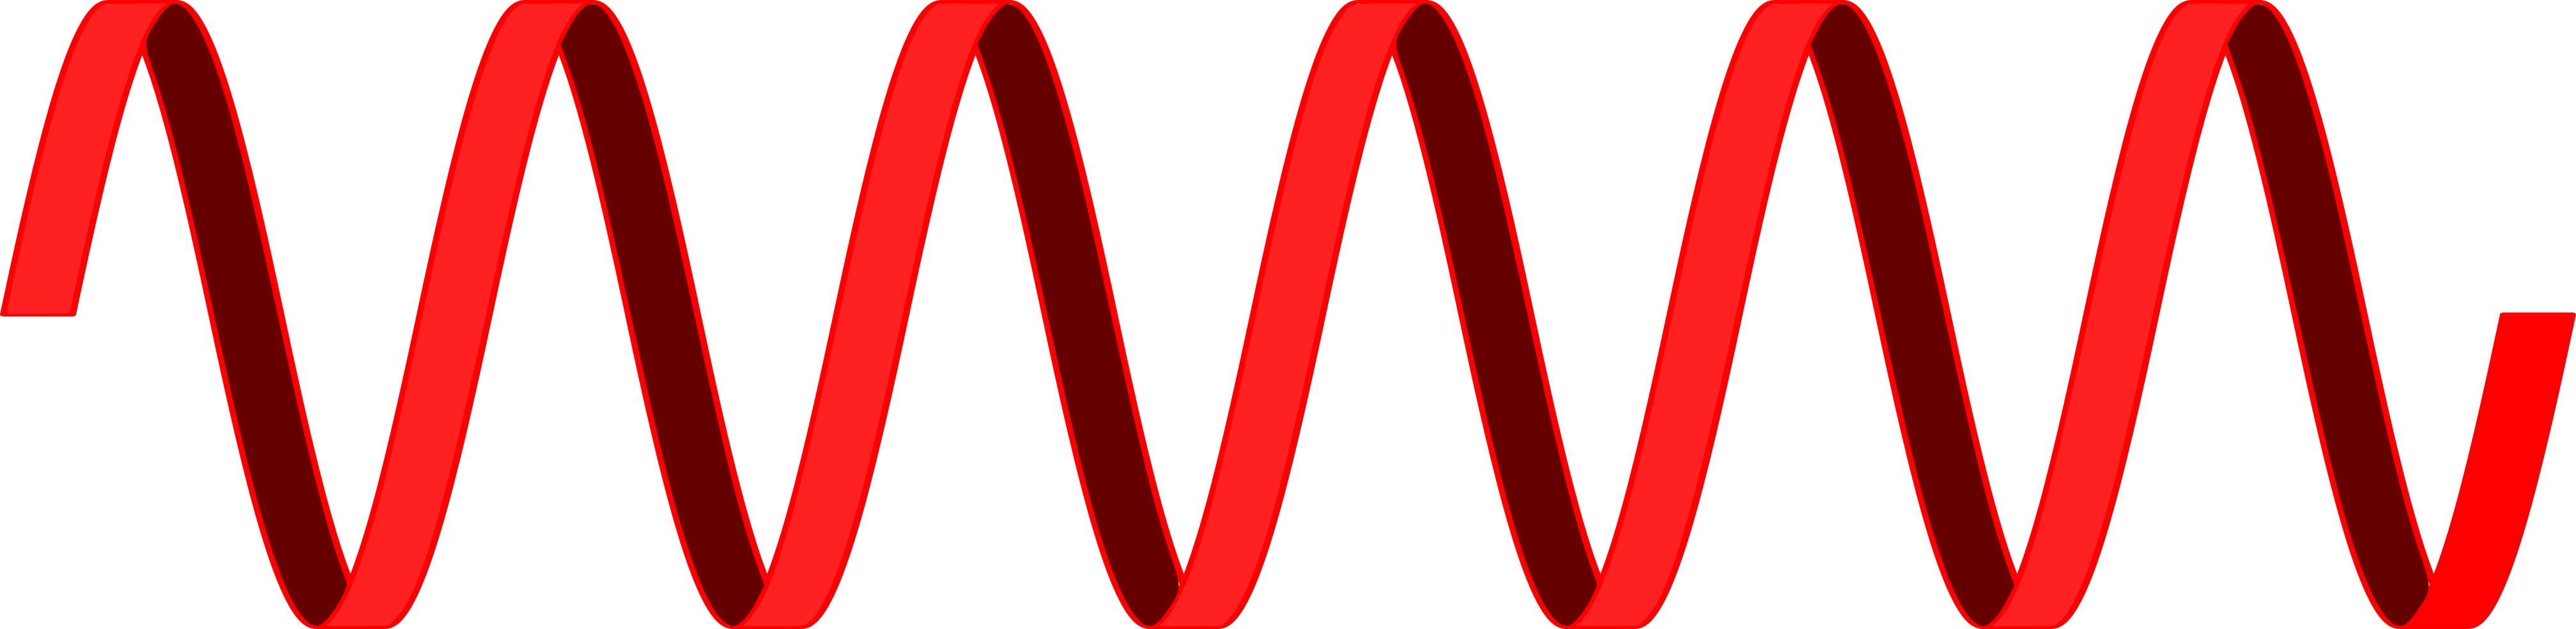
\includegraphics[width=\textwidth]{images/left_handed.png}
		\caption{}
		\label{fig:left_handed}
	\end{subfigure}
	\begin{subfigure}{0.49\textwidth}
		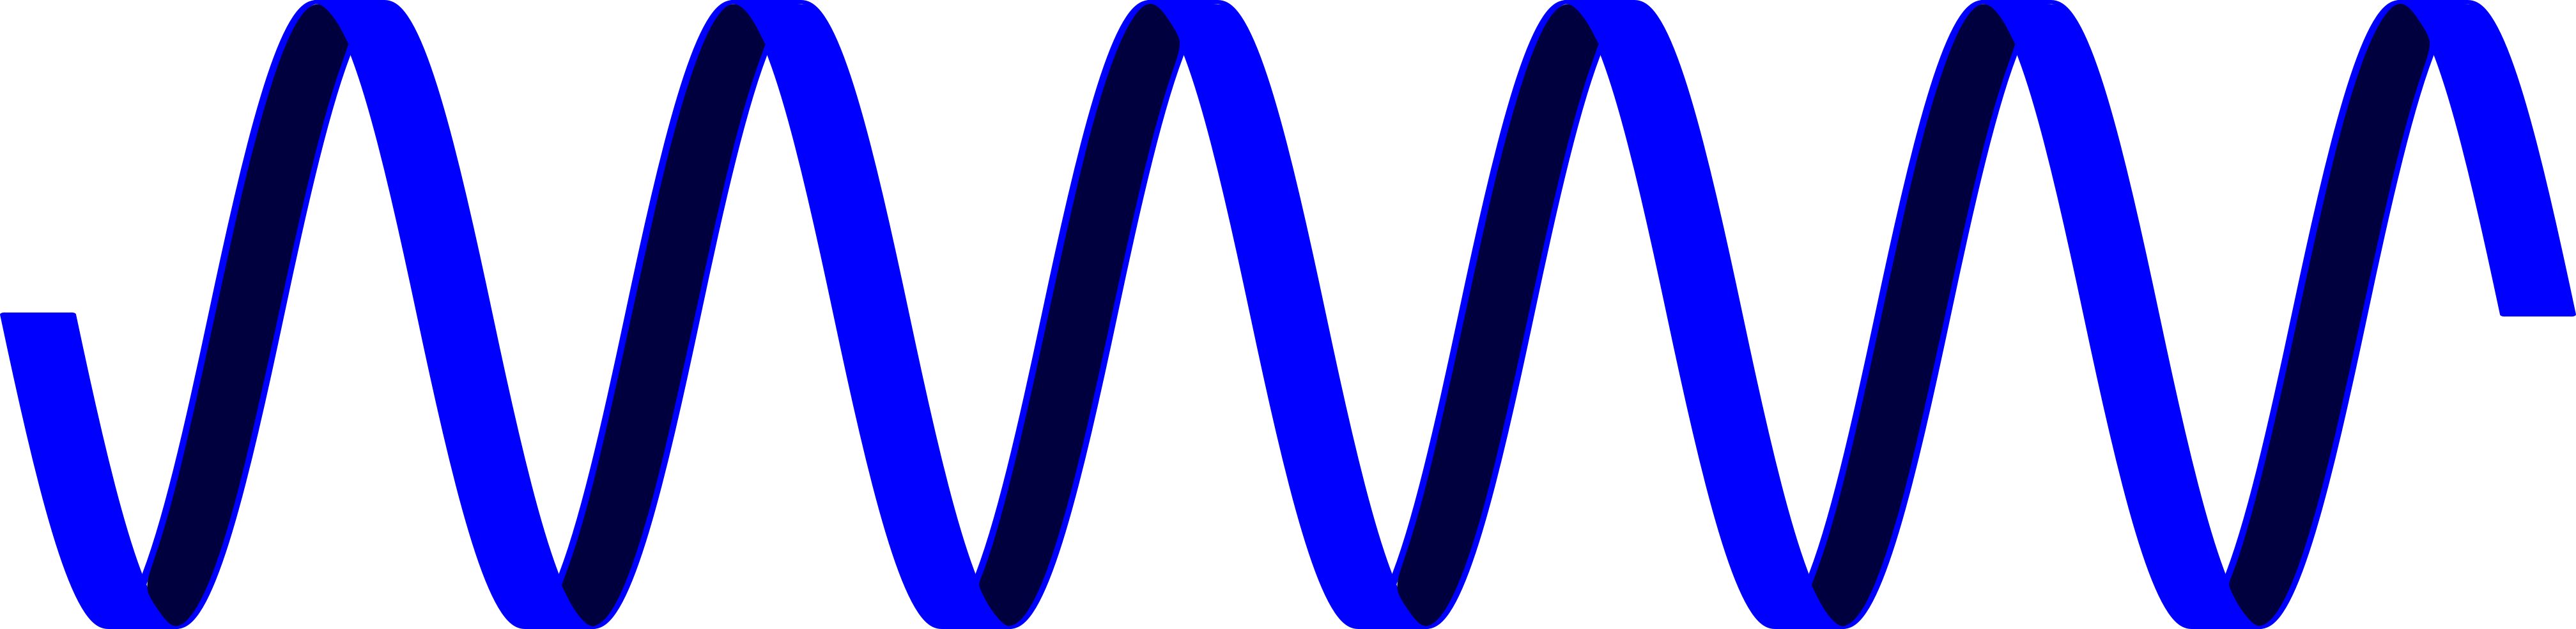
\includegraphics[width=\textwidth]{images/right_handed.png}
		\caption{}
		\label{fig:right_handed}
	\end{subfigure}
	\caption[Helix handedness]{\ref{fig:left_handed} Left handed helix. \ref{fig:right_handed} Right handed helix.}
	\label{fig:handedness}
\end{figure}

\subsection{Transfer matrices and bases for the field}

The cavity configurations explored in this report are described with the help of transfer matrices. Three bases are used to describe the field.
\begin{description}
	\item[Electromagnetic basis] The field is represented under the form $\left[E_x, E_y, H'_x, H'_y\right]^T$. Continuity of tangential components of the field allows to directly multiply two matrices describing two media to get the matrix describing the two media combined. However, this representation does not give a direct image of the components of the field propagating forward or backwards in the medium.
	\item[Cartesian basis] The field is written in the form $\left[E_x^+, E_y^+, E_x^-, E_y^-\right]^T$. This base allows to directly represent the field direction. However, the media studied induce circularly polarised field. This field is mainly used as a transition between electromagnetic and circular bases.
	\item[Circular basis] This is the basis of main interest for this study. The two main vectors are $\bm{e_1}$ and $\bm{e_2}$, given by equations \ref{eq:e1} and \ref{eq:e2}. The field is written $\left[E_L^+, E_R^+, E_L^-, E_R^-\right]^T$.
	\begin{eqnarray}
	\bm{e_1} &=& \frac{1}{\sqrt{2}}\begin{bmatrix}
	1\\i
	\end{bmatrix}\label{eq:e1}\\
	\bm{e_2} &=& \frac{1}{\sqrt{2}}\begin{bmatrix}
	1\\-i
	\end{bmatrix}\label{eq:e2}
	\end{eqnarray}
\end{description}
%
It is worth to note that $\bm{E}$ can be retrieved easily, independently from the medium \textit{via} equation \ref{eq:E}.
\begin{equation}
\bm{E} = \underbrace{E_L^+\bm{e_1}+E_R^+\bm{e_2}}_{=\begin{bmatrix}E_x^+\\E_y^+\end{bmatrix}}+\underbrace{E_L^-\bm{e_2}+E_R^-\bm{e_1}}_{=\begin{bmatrix}E_x^-\\E_y^-\end{bmatrix}}\label{eq:E}
\end{equation}
%
$\bm{H'}$ however is more difficult to calculate, and depends on the medium and the method used to simulate it.

\subsection{Partial inverse and reflection coefficients}
\label{sec:reflection}
One interesting feature of transfer matrices is that they allow the calculation of reflectivity quite easily, allowing to compare reflectivities with known results\cite{mccall_simplified_2009}. This subsection introduces a systematic way of expressing those coefficients, using partial inverses of matrices\cite{noauthor_partial_2020}.

If a matrix $\bm{M}$ links a state of light 0 to a state of light 1 (\textit{e.g.} for an interface or the propagation through a slab of chiral medium), \textit{i.e.} $\left[E_a, E_b, E_c, E_d\right]^T_{1} = \bm{M}\left[E_a, E_b, E_c, E_d\right]^T_{0}$, $\bm{M}$ can be rewritten by blocks
\begin{equation}
\begin{bmatrix}
E_a^+ \\
E_b^+ \\
E_a^- \\
E_b^- \\
\end{bmatrix}_{1} = \begin{pmatrix}
\bm{M_{11}} & \bm{M_{12}}\\
\bm{M_{21}} & \bm{M_{22}}\\
\end{pmatrix}\begin{bmatrix}
E_a^+ \\
E_b^+ \\
E_a^- \\
E_b^- \\
\end{bmatrix}_{0}
\end{equation}
By defining the partial inverse of $\bm{M}$, $\text{inv}_1(\bm{M})$, as
\begin{equation}
\text{inv}_1(\bm{M}) = \begin{pmatrix}
\bm{M_{11}}^{-1} & -\bm{M_{11}}^{-1}\bm{M_{12}}\\
\bm{M_{21}}\bm{M_{11}}^{-1} & \bm{M_{22}}-\bm{M_{21}}\bm{M_{11}}^{-1}\bm{M_{12}}\\
\end{pmatrix}
\end{equation}
We get
\begin{equation}
\begin{bmatrix}
E_{a,1}^+ \\
E_{b,1}^+ \\
E_{a,0}^- \\
E_{b,0}^- \\
\end{bmatrix} = \left(\text{inv}_1(\bm{M})\right)^{-1}\begin{bmatrix}
E_{a,0}^+ \\
E_{b,0}^+ \\
E_{a,1}^- \\
E_{b,1}^- \\
\end{bmatrix}\label{eq:pinv}
\end{equation}
Thus by knowing the boundary conditions $[E_{a,0}^+, E_{b,0}^+, E_{a,1}^-, E_{b,1}^-]^T$, it is possible to know the reflected and transmitted field $[E_{a,1}^+,E_{b,1}^+,E_{a,0}^-,E_{a,0}^-]^T$. 

By setting $[E_{a,1}^-, E_{b,1}^-] = \bm{0}$ in equation \ref{eq:pinv}\footnote{This no light is shone from the other side of the slab}, it is straightforward to see that the amplitude reflection and transmission coefficients associated to $\bm{M}$ are given by the first two columns of $\left(\text{inv}_1(\bm{M})\right)^{-1}$.
\begin{equation}
\left(\text{inv}_1(\bm{M})\right)^{-1} = \begin{pmatrix}
t_{aa} & t_{ab} & \ldots \\
t_{ba} & t_{bb} & \ldots \\
r_{aa} & r_{ab} & \ldots \\
r_{ba} & r_{bb} &  \ldots\\
\end{pmatrix}
\end{equation}
%
This allows to express directly the reflection and transmission coefficients.

\begin{eqnarray}
\begin{pmatrix}
t_{aa} & t_{ab} \\
t_{ba} & t_{bb}
\end{pmatrix} &=& \bm{M_{11}} - \bm{M_{12}}\bm{M_{22}}^{-1}\bm{M_{21}} \label{eq:transmission}\\
\begin{pmatrix}
r_{aa} & r_{ab} \\
r_{ba} & r_{bb}
\end{pmatrix} &=& -\bm{M_{22}}^{-1}\bm{M_{21}}\label{eq:reflection}
\end{eqnarray}

\subsection{Energy conservation}

From the reflection coefficients, it is possible to check energy conservation in the medium. Three criteria can be distinguished\cite{mccall_properties_2009}.  Expressing reflection coefficients in an arbitrary basis as in section \ref{sec:reflection}, equations \ref{eq:energyconservationa} and \ref{eq:energyconservationb} correspond to energy conservation for light incident to the medium with polarisation states $a$ and $b$ respectively. Equation \ref{eq:energyconservationredistribution} accounts for redistribution of energy between polarization states $a$ and $b$. $n1$ and $n2$ are the refractive indices of the isotropic media before and after the chiral medium.

\begin{eqnarray}
\abs{r_{aa}}^2+\abs{r_{ba}}^2+\left(\frac{n_2}{n_1}\right)(\abs{t_{aa}}^2+\abs{t_{ba}}^2)-1&=&0\label{eq:energyconservationa}\\
\abs{r_{ab}}^2+\abs{r_{bb}}^2+\left(\frac{n_2}{n_1}\right)(\abs{t_{ab}}^2+\abs{t_{bb}}^2)-1&=&0\label{eq:energyconservationb}\\
r_{aa}r_{ab}^*+r_{ba}r_{bb}^*+\left(\frac{n_2}{n_1}\right)(t_{aa}t_{ab}^*+t_{ba}t_{bb}^*) &=& 0 \label{eq:energyconservationredistribution}
\end{eqnarray}